	\chapter {Elektrostatika}


	\section{Uvodna razmatranja}
	U vrijeme antičke Grčke bile su poznate četiri pojave koje su povezane sa elektricitetom. To su munja, svjetlucanje oko šiljatih predmeta, ribe koje proizvode neku vrstu električnih udara i privlačenje laganih predmeta (slama) pomoću protrljanog komada ćilibara. Ove pojave su bile uočene, a sa elektricitetom povezane čitavih 2500 godina kasnije.

	\begin{marginfigure}%
		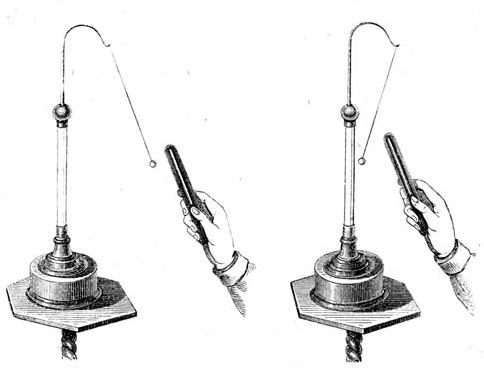
\includegraphics[width=\linewidth]{naboj}
		\caption{Naboj}
		\label{fig:naboj}
	\end{marginfigure}
	Aristotel (Aristotle, 384-322, pre n.e.) je opisao ribu torpiljarku ali nije uočio električni organ. Tales iz Mileta (Thalés Miléisos, oko 625-547. pre n.e.) je znao za privlačnu moć ćilibara koji su Sirijci zvali kamen kradljivac, a Perzijanci kradljivac slame (karuba). Grčki naziv elektor  ima značenje onaj koji privlači. U to vrijeme pominje se kamen linkurion, koji ima još veću moć privlačenja. Vjerovatno se radi o turmalinu ili topazu, jer se sa privlačenjem pominje i zagrijavanje kamena. U svim dokumentima iz tog perioda koji su sačuvani pominje se samo privlačenje. Odbojne sile tada nisu primijećene. Razlog za to je svuda prisutna gravitacija i znatno veće interesovanje za magnet koji privlači gvožđe, ma kako veliko bilo, dok ćilibar privlači različite, ali samo veoma lagane predmete. Takođe, pojava odbijanja nije mogla da se uklopi Aristotleovo učenje i učenje njegovih sljedbenika. Tek u šestom vijeku nove ere odbijanje kod magneta pominje Jovan Filopon. \\
	U periodu od 12, 13 vijeka Arapi su dali također veliki doprinos razvoju elektrostatike. U Evropi se značajnije pominje elektrostatia tek poslije.
	\begin{marginfigure}%
		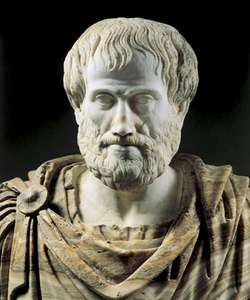
\includegraphics[width=\textwidth]{aristotle}
		\caption{Aristotel}
		\label{fig:aristotle}
	\end{marginfigure} 
	Naime, engleski ljekar Džilbert (William Gilbert 1544 – 1603) objavio je u svom djelu sistematsku raspravu o osobinama ćilibara da privlači vunu i rude magnetita da privlači gvožđe. On je Zemlju proglasio "velikim magnetom", 1630. godine je silu koja nastaje trenjem tijela nazvao \textit{vis electrica}.
	
	Za otkriće da elektricitet može da se kreće od jednog tijela do drugog zaslužan je Grej (Stephen Greu, 1670 – 1736), kao i za druge pojave. Godine 1733. došao je francuski fizičar de Faj (C. F. de Cisternay du Fay 1698 – 1739) do otkrića, da postoje dvije vrste elektriciteta, koje je nazivao staklasti i smolasti. 
	
	Tek 1975 godine je otkriven kondenzator u vidu staklene čaše sa naelektrisanim ekserom u njoj. Otkriće su predvodili Kleist i Mušenbruka. Ovaj eksperiment je ponovio Nole (Abbe Nollet) i dao ime uređaju Lajdenska boca. (Nikola Tesla: "Kleist i Mušenbruka su uspjeli da u bočicu zatvore tajanstvenu silu, koja iz bočice	bježi uz “ljuti” prasak, razvijajući rušilačku snagu. To je bilo rođenje kondenzatora, možda najčudesnije električne naprave koja je ikada pronađena").
	\begin{marginfigure}%
		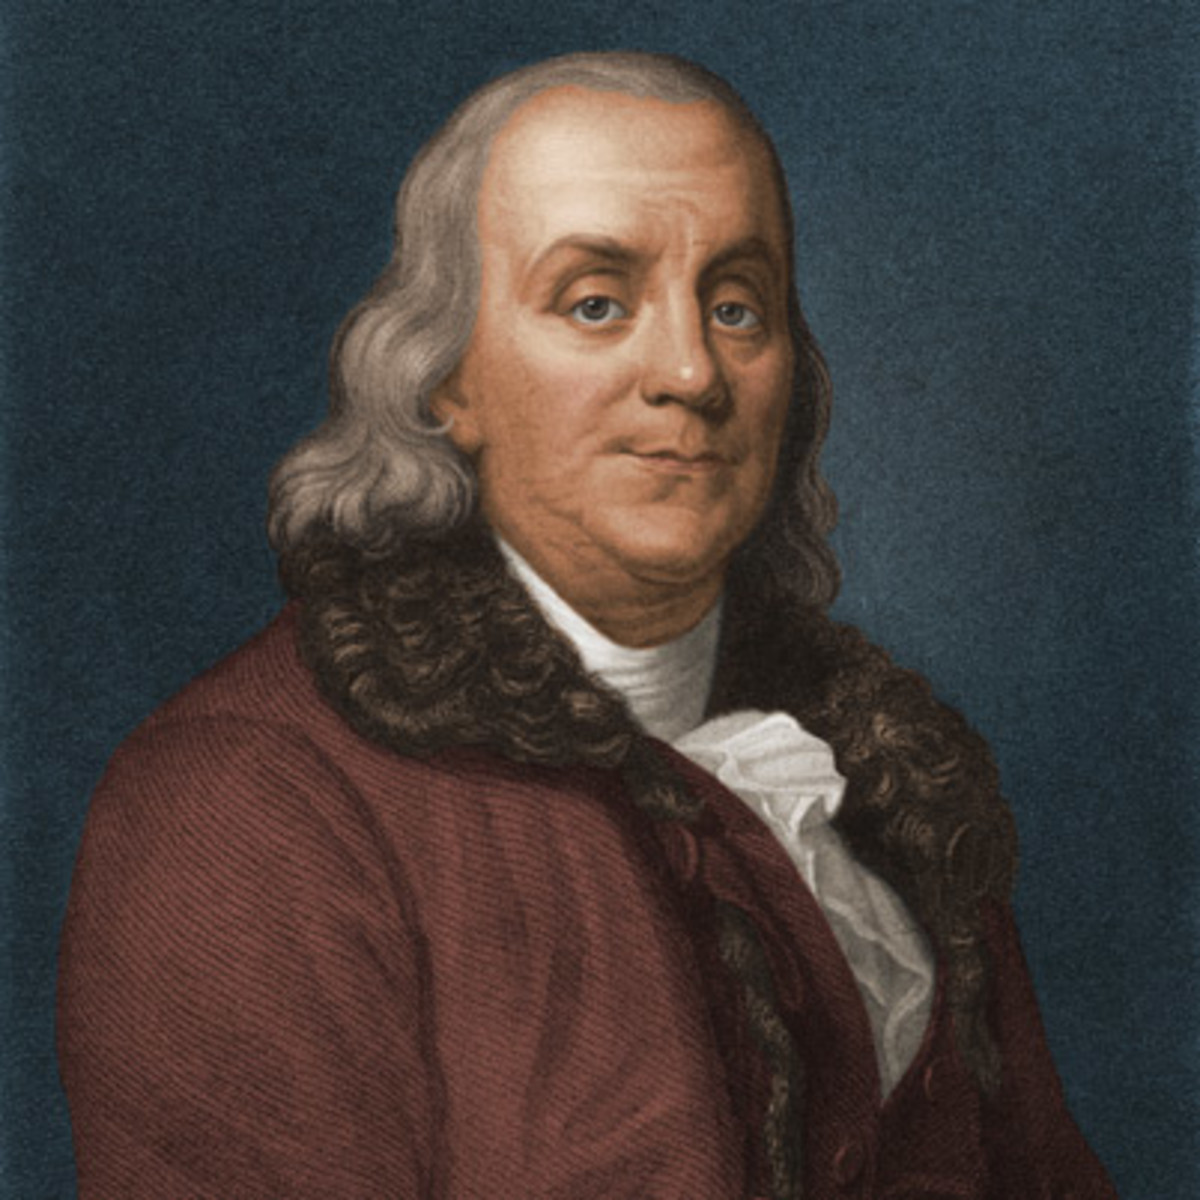
\includegraphics[width=\linewidth]{benjamin-franklin}
		\caption{Benjamin Frenklin}
		\label{fig:benjamin-franklin}
	\end{marginfigure} 
	Sjevernoamerički fizičar Benjamin Frenklin (1706 – 1790) je 1750. godine postavio
	prvu teoriju o prirodi elektriciteta: da je elektricitet fluid kojeg sva tijela imaju u određenoj količini. Benjamin Franklin je 1752. godine opisao grom kao električno pražnjenje i godinu kasnije pronašao gromobran. Godinu dana kasnije ruski fizičar Rihmen izvodio slične eksperimente, ali je prilikom toga poginuo od udara groma.\\
	Cijelo područje makroskopskih fenomena poznato pod nazivom elektrostatika osiguralo je istorijsku osnovu za razvitak koncepta elektrostatičkog naelektrisanja, kao mjerljive fizikalne veličine. Elektrostatika, jedno od glavnih područja nauke o elektricitetu, temelji se na samo jednom eksperimentalnom postulatu, inverznom kvadratnom zakonu, koji je jedan od fundamentalnih naučnih principa uopšte. Nije bio kreiran samo od jednog istraživača. 
	
	\begin{marginfigure}%
		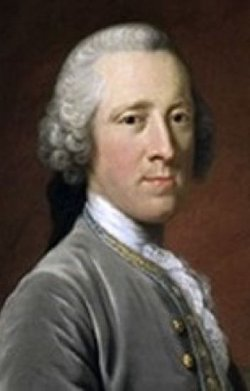
\includegraphics[width=\linewidth]{henry-kevendis}
		\caption{Henry Cavedish}
		\label{fig:kevendis}
	\end{marginfigure} 
	Prvi značajan doprinos dao mu je Benjamin Frenklin, a 1766. god. započeo je istraživanja Džozef Pristli (Joseph Priestley 1731 – 1804), na njegov podsticaj. Godine 1769. odredio je Robinson (J. Robinson 1739 – 1805) direktnim eksperimentom silu između električnih naelektrisanja, a Henri Kevendiš (Henry Cavendish 1731 – 1810) je 1773. definitivno potvrdio taj zakon. \\

	\begin{marginfigure}%
		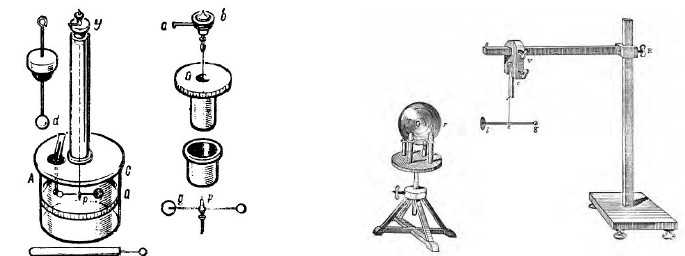
\includegraphics[width=\linewidth]{kulonova}
		\caption{Kulonova torziona vaga i uređaj za različita naelektrisanja}
		\label{fig:kulonova}
	\end{marginfigure}
	Kako je ustanovljeno da postoje dvije vrste naelektrisanja, pozitivno i negativno, što uslovljava privlačenje i odbijanje naelektrisanih tijela Kulon (Charles Augustin Koulon 1736 - 1860) je svojim radovima dao opšti zakon međusobnog djelovanja naelektrisanih tijela na nekom rastojanju. On je 1785. godine demonstrirao inverzni kvadratni zakon, pomoću precizne torzione vage, kojom mogu da se mjere veoma male sile. Ova vaga je dobila ime po njemu Kulonova torziona vaga.\\
	
	
	Njegova otkrića čine prvu kvantitativnu bazu za matematički prikaz zakona električne sile, koji utvrđuje da dva električno naelektrisana tijela, čija veličina je mala u odnosu na udaljenost između njih, djeluju jedno na drugo s jednakim i suprotnim silama, koje su obrnuto srazmjerne kvadratu njihove međusobne udaljenosti. Kulonova metoda eksperimentalnog određivanja inverznog kvadratnog zakona bila je direktna, kvantitativna i lahko razumljiva, pa su njegovi rezultati bili spremno prihvaćeni. To su prvi rezultati iz nauke o elektricitetu, koji su bili objavljeni i široko rasprostranjeni. \\
	\begin{marginfigure}%
		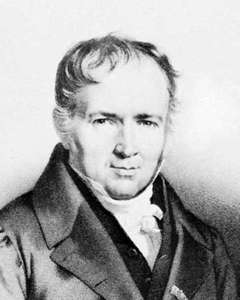
\includegraphics[width=\linewidth]{poisson}
		\caption{Simeon Denis Poisson 1781 – 1840}
		\label{fig:poisson}
	\end{marginfigure} 
	Tome su znatno	doprinijela i teoretska razmatranja S. Poasona, objavljena u dva memoara 1812. i 1813. godine. U njima je on, uzimajući Kulonov inverzni kvadratni zakon kao fundamentalni postulat, znatno unaprijedio i upotpunio elektrostatiku upotrebom analogije prema gravitacionoj teoriji, koja je tada bila visoko razvijena. S. Poason je, na osnovu Kulonovog zakona, uveo funkciju $ \Phi(x,y,z) $ , kojoj doprinose sva naelektrisanja jednog električnog sistema obrnuto proporcionalno s udaljenošću. Petnaest godina kasnije u generalisanju Poasonovih radova o električnim i magnetnim pojavama, Grin (1731 – 1841) daje funkciji $ \Phi $ univerzalno ime \textit{potencijal}.\\
	
		
		
	Voltin (Alessandro Volta 1745 – 1827) pronalazak prve hemijske baterije bio je neposredan podsticaj i za studij vođenja elektriciteta. Značajne rezultate u istraživanju vođenja postigli su Hamfri Dejvi (Humphry Davy 1778 – 1829) i Om (George Simeon Ohm 1787 – 1854). \\
	
	\begin{marginfigure}%
		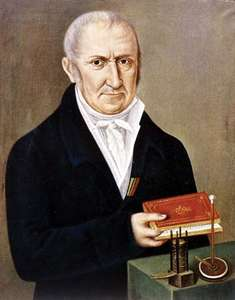
\includegraphics[width=\linewidth]{volta}
		\caption{Alessandro Volta}
		\label{fig:volta}
	\end{marginfigure} 

	Om je 1826. godine formulisao rezulta eksperimentalnih istraživanja, da je jačina struje u žici koja ne sadrži nikakvu elektromotornu silu proporcionalna razlici potencijala na njenim krajevima. Ta činjenica, iako ne spada u posebnu klasu zakona nezavisnih od materije, nazvana je Omovim zakonom. Zakon je u suštini vrlo jednostavan, no mora se upotrebljavati s pažnjom. Upravo zbog njegove jednostavnosti, trebalo je proći oko 14 godina, pa da to veliko otkriće u naučnom svijetu bude priznato i prihvaćeno. Godine 1841. Džul (J. P. Joule 1818 – 1889) utvrđuje zakon koji povezuje struju koja protiče metalnim provodnikom s razvijenom toplotom u njemu.\\
	
	
	\begin{marginfigure}%
		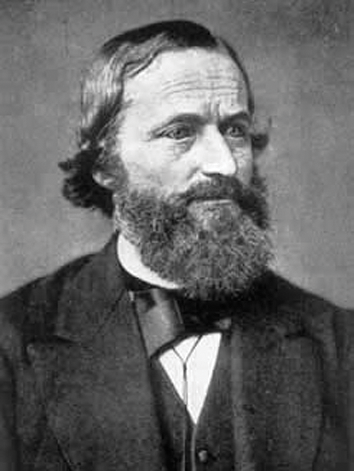
\includegraphics[width=\linewidth]{kirhof}
		\caption{Gustav Robert Kirchhoff 1824 – 1887}
		\label{fig:kirhof}
	\end{marginfigure} 
	
	Veliki napredak u istraživanju električnog strujanja u provodnicima zabilježen je 1847. godine, kada je Kirhof dedukcijom izveo i formulisao svoja dva zakona, koji spadaju u grupu temeljnih zakona klasične elektromagnetne teorije. \\
	Prvi Kirhofov zakon govori o  kontinuitetu električne struje, dok je drugi Kirhofov zakon matematički identičan sa zakonom da razlika potencijala između bilo kojih dviju tačaka ima istu vrijednost po svim putevima između njih. Ovi zakoni su vrlo korisni i mnogo su upotrebljavani u elektrotehnici. Imali su velikog značaja u njenom napretku i posebno su značajni za razvoj električnih krugova i mreža.